\section{Premier étude des conditions aux limites transparentes}
\label{sec:TBC}

\subsection{Introduction et quelques exemples de motivation}

\indent Le contenu présenté dans cette section est une introduction aux objectifs qu'on envisage dans ce stage, concernant l'étude des conditions aux limites transparentes (en anglais, \emph{transparent boundary conditions} - TBCs) afin de les appliquer à des méthodes de décomposition de domaine (en anglais, \emph{domain decomposition methods} - DDMs) . Cet étude a été développé sur l'équation de KdV, parce que c'était, parmi les modèles étudiés et implémentés jusqu'au moment où on a commencé cette partie du projet, celui pour lequel on a obtenu la meilleure et plus fiable implémentation numérique. En plus, la linéarisation de l'équation de KdV est plus évidente que pour les équations de Serre - comme on discutera plus tard, l'étude des TBCs pour des équations linéaires est beaucoup plus développé que pour les non linéaires.

\indent Les TBCs sons construites de façon que la solution calculée dans le domaine computationnel fini $\Omega$ coïncide avec la solution du problème dans tout l'espace, restreinte à $\Omega$. En général, ces conditions aux bords son non locales en temps, alors elles doivent être approximées pour permettre une implémentation numérique efficiente \cite{Xavieretal2008}.

\indent Pour le problème

\begin{equation*}
\begin{cases}
\mathcal{A}(u) = f \ \ \text{in} \ \ \Omega\\
u = 0 \ \ \text{on} \ \ \partial\Omega\\
\end{cases}
\end{equation*}

\noindent où $\mathcal{A}$ est un opérateur différentiel partiel, les TBCs exactes dans $\Gamma \subset \partial\Omega$ (par example, dans une DDM, $\Gamma$ est l'interface entre deux subdomaines) sont données par \cite{Japhet2003}

\begin{equation}
\label{eq:exactTBC}
B(u) = \frac{\partial}{\partial n}u + D2N(u) = 0
\end{equation}

\noindent où $\partial n$ est le vecteur normal sortant à $\Omega$ sur $\Gamma$ , et l'opérateur D2N (\emph{Dirichlet to Neumann}) est défini par

$$\left. D2N : \alpha(x) \mapsto \frac{\partial}{\partial n^c}v \right\rvert_{\Gamma}$$

\noindent avec $\alpha$ défini sur $\Gamma$ et $\partial n^c$ étant le vecteur normal sortant au complémentaire de $\Omega$, dénoté $\Omega^c$. $v$ est solution du problème suivant, résolu dans $\Omega^c$ : 

\begin{equation*}
\begin{cases}
\mathcal{A}(v) = f \ \ \text{in} \ \ \Omega^c\\
v = 0 \ \ \text{on} \ \ \partial \Omega^c \backslash \Gamma \\
v = \alpha \ \ \text{on} \ \ \Gamma
\end{cases}
\end{equation*}

\indent Ainsi, on peut interpréter interpréter l'opérateur D2N comme une imposition de continuité de la dérivée de la solution dans la direction normale à l'interface. Par ailleurs, comme son nom indique, cet opérateur construit une dérivée (une condition de Neumann) à partir de la solution dans $\Omega^c$ (une condition de Dirichlet).



\indent Présentons d'abord un example simple, dont la solution y la TBC analytiques sont connues. On va considérer le problème 1D suivant :

\begin{equation*}
\begin{cases}
-u''(x) = 1 \ \ in \ \ \Omega = [0,2]\\
u(0) = 0 \\
u(2) = 0
\end{cases}
\end{equation*}

\noindent dont la solution est

$$u(x) = -\frac{x^2}{2} + x$$

\noindent et, en considérant la partition de $\Omega$ en $\Omega_1 = [0,1]$ et $\Omega_2 = [1,2]$, on va considérer le problème

\begin{equation*}
\begin{cases}
-u_1''(x) = 1 \ \ in \ \ \Omega_1\\
u_1(0) = 0 \\
\mathcal{B}(u_1) = 0 \ \ at \ \ \Gamma=\{1\}
\end{cases}
\end{equation*}

\noindent où la TBC $\mathcal{B}(u)$ est telle que $u|_{\Omega_1} = u_1$.

\indent La fonction $v$, pour la détermination de l'opérateur D2N, est solution de

\begin{equation*}
\begin{cases}
-v''(x) = 1 \ \ in \ \ \Omega_2\\
v(2) = 0 \\
v(1) = \alpha \ \ at \ \ \Gamma=\{1\}
\end{cases}
\end{equation*}

\noindent alors

$$v(x) = -\frac{x^2}{2} + \left(\frac{3}{2} - \alpha \right) + 2\alpha -1$$

\noindent et

$$\left. \frac{\partial}{\partial x}v \right\rvert_{x=1} = \frac{1}{2} - \alpha$$

\indent Finalement, la TBC, dans la forme \eqref{eq:exactTBC}, s'écrit

$$B(u_1) = \frac{\partial}{\partial x}u_1 + D2N(u_1) = \frac{\partial}{\partial x}u_1+ \frac{1}{2} - u_1$$

\indent Le problème a été résolu avec une méthode de différences finies, avec des approximations centrées de seconde ordre pour la dérivée spatiale, dans deux grilles différentes. La figure \ref{fig:TBClaplace} montre que la TBC construite fournit effectivement une solution convergente à la solution de référence restreinte à $\Omega$.

\begin{center}
	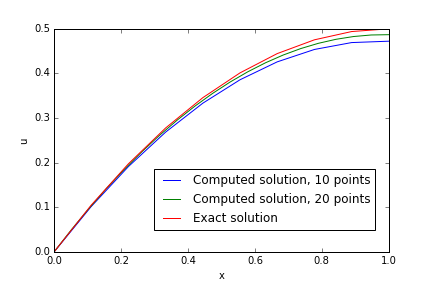
\includegraphics[scale=.5]{figures/TBClaplace.png}
	\captionof{figure}{Solutions pour l'équation de Laplace avec TBC \label{fig:TBClaplace}}
\end{center}

\indent En retournant aux modèles d'ondes, on rappelle que, dans les premières simulations avec la méthode de \emph{splitting} adoptée pour la résolution de l'équation de KdV, on n'a pas utilisé une application rigoureuse  de conditions aux bords appropriées. En fait, notre objectif principal était la validation de la méthode; alors, en imposant des conditions périodiques ou des conditions de Dirichlet ou Neumann homogènes, on a analysé l'évolution de la solution seulement avant son arrivée aux bords.

\indent Avant de commencer l'étude des TBCs pour l'équation de KdV, on va présenter deux examples de motivation à ce travail. Le premier exemple montre très clairement l'influence de conditions aux bords inappropriées sur la solution. On a résolu deux fois le mème problème, avec la même solution initiale, conditions aux bords et discrétisations spatiales et temporales :

\begin{equation*}
    \begin{cases}
    u_t + u_x + (u^2)_x + u_{xxx} = 0 \ , \ \ x \in \Omega=[a,b] \ \ t \in [0, t_{max}] \\
    u(x,0) = \Phi(x) \\
    u(a,t) = 0 \\
    u(b,t) = 0 \\
    u_x(b,t) = 0  \\ 
    \end{cases}
\end{equation*}

\indent La seule différence entre les deux problèmes est la taille de ses domaines: ils ont été choisis de façon que l'onde arrive aux bords (dans le temps de simulation) dans le première problème, mais pas dans le deuxième. La figure \ref{fig:motivational1} montre comme la différence entre les deux solutions augmente avec le temps, en partant du bord et se propageant pour tout le domaine:

\begingroup
	\noindent
	\begin{minipage}[t]{.3\linewidth}
		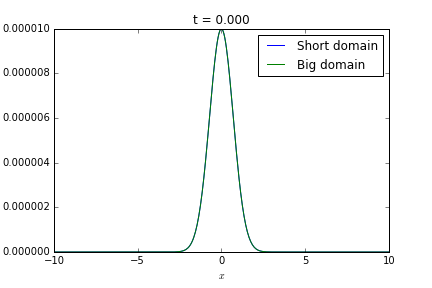
\includegraphics[scale=.3]{figures/motivational1A.png}	
	\end{minipage}
	\hfill
	\begin{minipage}[t]{.3\linewidth}
		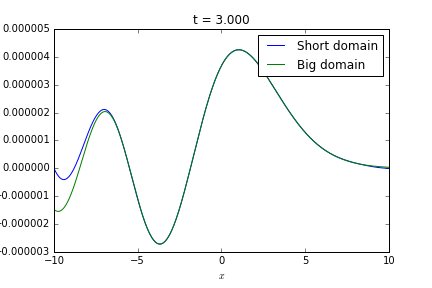
\includegraphics[scale=.3]{figures/motivational1B.png}	
	\end{minipage}
	\hfill
	\begin{minipage}[t]{.3\linewidth}
		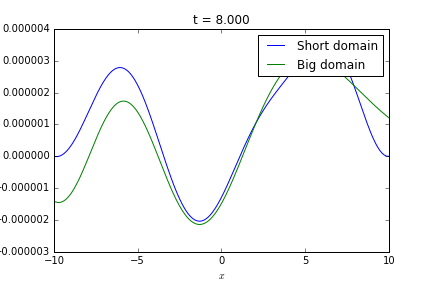
\includegraphics[scale=.3]{figures/motivational1C.png}	
	\end{minipage}
	\captionof{figure}{Premier exemple de motivation : comparaison entre les solutions dans un petit domaine (en bleu) et un large domaine (en vert) \label{fig:motivational1}}
\endgroup

\indent Alors, on cherche des conditions aux bords qui puissent bien simuler les TBCs, c'est-à-dire, de façon que la solution calculé dans $\Omega$ soit le même que la solution de tout le domaine restreinte à $\Omega$. Par conséquent, on veut des bords qui n'ont pas d'influence sur la solution, permettant qu'elle puisse simplement "sortir" du domaine.

\indent L'exemple suivant montre une deuxième motivation pour ce travail. On veut résoudre le problème 

\begin{equation*}
    (P_1) \begin{cases}
    u_t + u_x + (u^2)_x + u_{xxx} = 0 \ , \ \ x \in \Omega_1 = [0,L], \ \ t \in [0, t_{max}] \\
    u(x,0) = \Phi(x) \\
    u(0,t) = 0 \\
    u_x(0,t) = 0 \\
    u(L,t) = g(t)  \\ 
    \end{cases}
\end{equation*}

\indent On cherche une fonction  $g(t)$ pour simuler le TBC. Pour atteindre cet objectif, on va d'abord résoudre le problème

\begin{equation*}
    (P_2) \begin{cases}
    u_t + u_x + (u^2)_x + u_{xxx} = 0 \ , \ \ x \in \Omega_2 = [0,2L], \ \ t \in [0, t_{max}] \\
    u(x,0) = \Phi(x) \\
    u(0,t) = 0 \\
    u_x(0,t) = 0 \\
    u(2L,t) = 0  \\ 
    \end{cases}
\end{equation*}

\noindent (\emph{i.e.}, la même équation résolue dans un domaine plus grand) et on impose $g(t) = u_2(t)$, où $u_2$ est la solution de $(P_2)$. Afin d'obtenir des résultats plus précis, les deux calculs sont réalisés avec les mêmes pas de temps et taille du maillage.

\indent Supposons qu'il y a une unique solution $u_1$ pour $(P_1)$. On peut facilement voir que $u_2|_{\Omega_1}$ est également solution de $(P_1)$. Alors, $u_1 = u_2|_{\Omega_1}$. Ce fait justifie pourquoi notre procédure marche comme une TBC, en fournissant la solution "exacte", comme montre la figure \ref{fig:motivation2}  (détail sur la région proche du bord droit).

\begingroup
\noindent
	\begin{minipage}{.45\linewidth}
		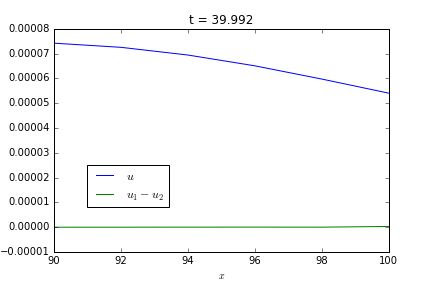
\includegraphics[scale=.5]{figures/motivational2A.png}	
	\end{minipage}
	\hfill
	\begin{minipage}{.45\linewidth}
		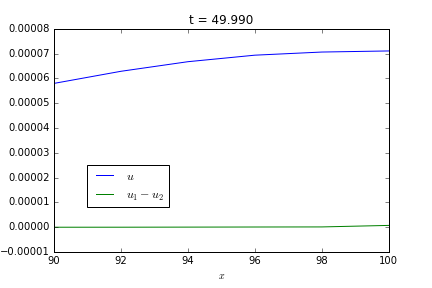
\includegraphics[scale=.5]{figures/motivational2B.png}	
	\end{minipage}
	\captionof{figure}{Deuxième exemple de motivation : solution avec une condition de Dirichlet "exacte" sur le bord à droite \label{fig:motivation2}}
\endgroup

\subsection{Optimisation de conditions aux limites de Robin pour simuler des TBCs}

\indent La procédure présentée dans le dernier example ne peut pas être appliquée en pratique. En fait, calculer la solution dans un domaine plus grand et l'utiliser comme solution exacte pour construire les conditions aux bords n'est qu'une "triche". Alors, on veut plutôt déterminer des approximations pour les TBCs sans avoir une solution de référence. Ces conditions approximées seront des conditions de Robin, en utilisant la valeur de la solution et de ses dérivées au bord.

\subsubsection{Conditions aux limites de Robin jusqu'à la dérivée première}

\indent Dans un approche initial, l'équation de KdV sera résolue dans le domaine $[-L,L]$ avec les conditions aux bords suivants (imposés dans la résolution du deuxième pas de la méthode de \emph{splitting}):

\begin{equation*}
\begin{cases}
    u(-L) = 0 \\
    u_x(-L) = 0 \\
    \alpha u(L) + \beta u_x(L) = 0,  \ \ \alpha,\beta > 0
\end{cases}
\end{equation*}

\indent La troisième condition aux bords consiste en des conditions de Robin, avec des paramètres $\alpha$ et $\beta$ (ou, de façon équivalente, le paramètre  $\beta/\alpha$) qui seront optimisés afin de simuler une TBC sur le bord à droite. Dans un premier moment, on va considérer des conditions de Robin contenant jusqu'à la première dérivée de la solution.

\indent Afin de trouver les coefficients optimaux, on va tester plusieurs paires $(1,\beta/\alpha)$ (y compris les limites $\beta/\alpha \rightarrow 0$ et $\beta/\alpha \rightarrow \infty$, correspondant respectivement aux conditions de Dirichlet et de Neumann) et calculer l'erreur par rapport à la solution de référence $u_{ref}$, calculée dans le domaine $[-2L,2L]$. Deux erreurs seront calculées, pour chaque pas de temps $t_n$ :

\begin{equation*}
e_1^n = \sqrt{\sum_{i=0}^N{\left( u^n_i - (u_{ref})^n_i\right)^2}} \qquad
e_2^n =  u^n_N - (u_{ref})^n_N
\end{equation*}

\indent $e_2^n$ est calculé pour montrer que la plus grande partie de l'erreur $e_1^n$ de tout le domaine est due aux bords.
 
\indent Les figures \ref{fig:robin1} à \ref{fig:robinErrorsExample} montrent la solution dans quelques instants et l'évolution de $e_1$ et $e_2$ pour certains valeurs de $\beta/\alpha$. La figure \ref{fig:robinErrorsAll} compare $e_2$  pour plusieurs autres valeurs, y compris le cas de pure Dirichlet  (avec $\alpha = 1, \beta = 0$, alors $log(\beta/\alpha) = -\infty$) et pure Neumann (avec $\alpha = 0, \beta = 1$).

\begingroup
	\noindent
	\begin{minipage}{.45\linewidth}
		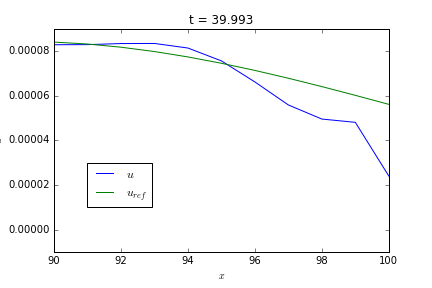
\includegraphics[scale=.5]{figures/robin1A.png}	
	\end{minipage}
	\hfill
	\begin{minipage}{.45\linewidth}
		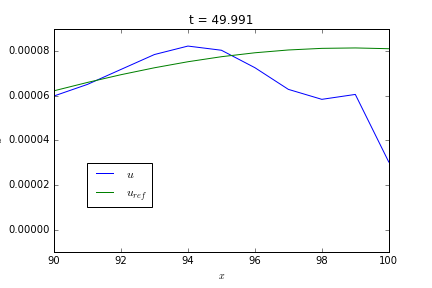
\includegraphics[scale=.5]{figures/robin1B.png}	
	\end{minipage}
	\captionof{figure}{Solution de référence et solution approximée pour  $\beta/\alpha = 1$ \label{fig:robin1}}
\endgroup

\begingroup
\noindent
	\begin{minipage}{.45\textwidth} 
		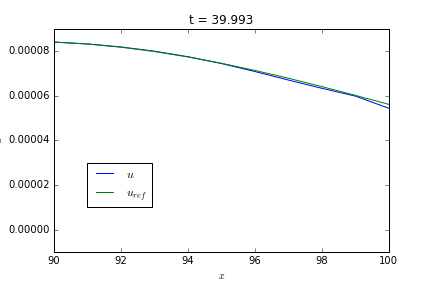
\includegraphics[scale=.5]{figures/robin10A.png}	
	\end{minipage}
	\hfill
	\begin{minipage}{.45\linewidth}
		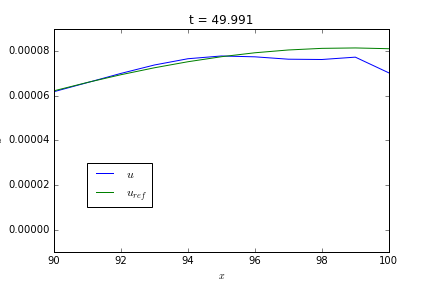
\includegraphics[scale=.5]{figures/robin10B.png}	
	\end{minipage}
	\captionof{figure}{Solution de référence et solution approximée pour  $\beta/\alpha = 10$ \label{fig:robin10}}
\endgroup

\begingroup
\noindent 
	\begin{minipage}{.45\textwidth} 
		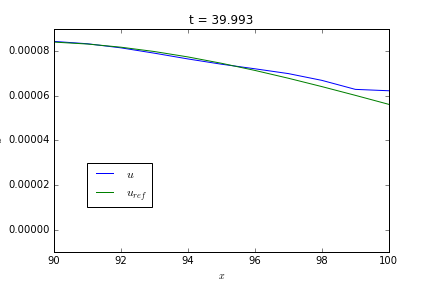
\includegraphics[scale=.5]{figures/robin100A.png}	
	\end{minipage}
	\hfill
	\begin{minipage}{.45\linewidth}
		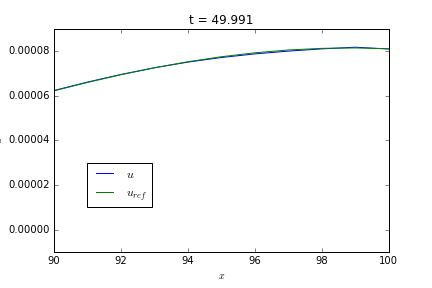
\includegraphics[scale=.5]{figures/robin100B.png}	
	\end{minipage}
	\captionof{figure}{Solution de référence et solution approximée pour  $\beta/\alpha = 100$ \label{fig:robin100}}
\endgroup

\begingroup
\noindent
	\begin{minipage}{.3\textwidth} 
		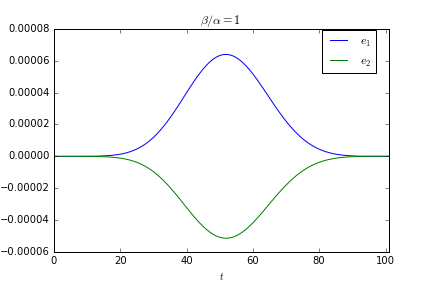
\includegraphics[scale=.3]{figures/robin1Error.png}	
		\captionof{subfigure}{$\beta/\alpha = 1$}
	\end{minipage}
	\hfill
	\begin{minipage}{.3\textwidth} 
		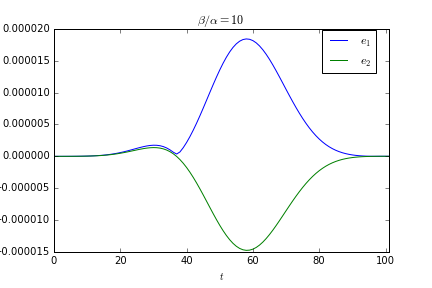
\includegraphics[scale=.3]{figures/robin10Error.png}	
		\captionof{subfigure}{$\beta/\alpha = 10$}
	\end{minipage}
	\hfill
	\begin{minipage}{.3\textwidth}
		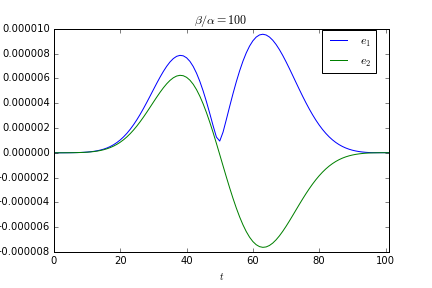
\includegraphics[scale=.3]{figures/robin100Error.png}	
		\captionof{subfigure}{$\beta/\alpha = 100$}
	\end{minipage}
	\captionof{figure}{Erreurs entre la solution approximée et la solution de référence \label{fig:robinErrorsExample}}
\endgroup

\begingroup
\begin{center}
		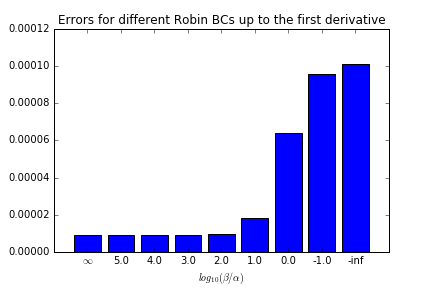
\includegraphics[scale=.6]{figures/robinErrors1.png}
	     \captionof{figure}{Erreur $||e_1| = \sum_{n=0}^{n_{max}}(e^n_1)^2$ entre la solution approximée et la solution de référence pour des plusieurs valeurs de $\beta/\alpha$, avec des conditions aux limits de Robin jusqu'à la dérivée première \label{fig:robinErrorsAll}}
\end{center}
\endgroup

\indent Les résultats présentés dans les figures \ref{fig:robin1} jusqu'à \ref{fig:robinErrorsAll} montrent que des conditions aux bord avec un caractère de Neumann plus fort produisent des meilleures approximations pour la TBC, en comparaison à des conditions plus proches du pure Dirichlet. Les résultats pour le pure Neumann et pour le Neumann avec un petit mais pas nul Dirichlet terme sont très proches, comme présenté dans le tableau \ref{tab:robinErrorsZoom} pour un étude plus raffiné autour des meilleures valeurs de $\beta/\alpha$. En fait, imposer la solution nulle aux bord est une condition trop forte, et la condition de Neumann peut capturer de façon plus satisfaisant la lisseté de la solution.

\begingroup
\begin{center}
		\begin{tabular}{c|c}
			$log(\beta/\alpha)$ & Error ($\times 10^{-6}$) \\
			\hline
			2.5 & 8.93\\
			3.0 & 8.87\\
			3.5 & 8.95\\
			4.0 & 8.98\\
			4.5 & 8.99\\
			5.0 & 8.99\\
			$\infty$ & 8.99	
		\end{tabular}
		\captionof{table}{Erreur $||e_1| = \sum_{n=0}^{n_{max}}(e^n_1)^2$ pour quelques valeurs de $\beta/\alpha$ autour des meilleurs résultats \label{tab:robinErrorsZoom}}
\end{center}
\endgroup

\subsubsection{Conditions aux limites de Robin jusqu'à la dérivée seconde}

\indent On a répété les tests décrits ci-dessus, mais en remplaçant les conditions au bord droit par $\alpha u(L) + \beta u_x(L) + \gamma u_{xx}(L) = 0,  \ \ \alpha,\beta, \gamma > 0$.

\indent Les valeurs de $\alpha$ et $\beta$ sont fixés et égaux à celui qui a donné l'erreur minimal dans les simulations précédentes ($(\alpha,\beta) = (1,1000)$). On montre directement le graphe contenant les erreurs pour des plusieurs valeurs de $\gamma/\beta$ (figure \ref{fig:robinErrorsAll2}). De façon similaire aux conclusions faites ci-dessus, on a observé une meilleure approximation de la TBC pour des valeurs plus fortes de $\gamma/\beta$ (étant l'erreur presque constant à partir d'un certain seuil, comme montre le tableau \ref{tab:robinErrors2Zoom}). En fait, même l'erreur le plus grande dans la figure \ref{fig:robinErrorsAll2} ($||e_1||(\gamma/\beta = 0.01) = 8.78 \times 10^{-6}$) est plus petit que le meilleur cas présenté dans le tableau \ref{tab:robinErrorsZoom}.

\begingroup
\begin{center}
		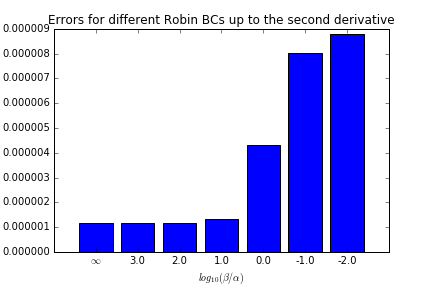
\includegraphics[scale=.6]{figures/robinErrors2.png}
	     \captionof{figure}{Erreur $||e_1| = \sum_{n=0}^{n_{max}}(e^n_1)^2$ entre la solution approximée et la solution de réference pour des plusieurs valeurs de $\gamma/\beta$, avec des conditions aux limits de Robin jusqu'à la dérivée seconde  \label{fig:robinErrorsAll2}}
\end{center}
\endgroup

\begingroup
\begin{center}
		\begin{tabular}{c|c}
			$log(\gamma/\beta)$ & Error ($\times 10^{-6}$) \\
			\hline
			2.0 & 1.157665\\
			2.5 & 1.157382\\
			3.0 & 1.157280\\
			3.5 & 1.157247\\
			4.0 & 1.157236\\
			4.5 & 1.157233\\
			$\infty$ & 1.157231	
		\end{tabular}
		\captionof{table}{Error $||e_1| = \sum_{n=0}^{n_{max}}(e^n_1)^2$ for some values of $\gamma/beta$ around the best ones \label{tab:robinErrors2Zoom}}
\end{center}
\endgroup

\subsubsection{Conclusion partiale} 

\indent Pour résumer cet étude initial des conditions transparentes, on a cherché à les approximer par des conditions aux bords de Robin, écrites en fonction de coefficients ajustables afin d'attribuer différentes importances à chacun des termes (correspondant à la solution et à ses dérivées). L'idée était de tester plusieurs combinaisons de ces coefficients afin de les optimiser (au sens de minimiser l'erreur entre la solution calculée dans $[-L,L]$ et la solution de référence, calculée dans $[-2L,2L]$). Comme on a décrit ci-dessus, les conditions de Robin qui prennent en compte la continuité de la solution testée (i.e., avec des coefficients plus grands pour les termes des dérivées) ont produit des meilleurs résultats. Alors, la TBC basée sur la première dérivée a été plus efficiente que celle basée seulement sur la solution; et la TBC basée sur la seconde dérivée a été encore meilleure. Finalement, on a observé que l'amélioration de la solution est négligeable au-dessus une certaine relation entre les coefficients.
















